%% rnaastex.cls is the classfile used for Research Notes. It is derived
%% from aastex61.cls with a few tweaks to allow for the unique format required.
\documentclass[rnaas]{aastex62}

%% Define new commands here
\newcommand\latex{La\TeX}

\newcommand{\tess}{{\it TESS}}
\newcommand{\wf}{{\it WFIRST}}

\usepackage{hyperref}

\newcommand{\chicago}{Department of Astronomy and Astrophysics, University of
Chicago, 5640 S. Ellis Ave, Chicago, IL 60637, USA}
\newcommand{\sagan}{Sagan Fellow}

\begin{document}

\title{Unbiased inference of the masses of transiting planets from radial velocity followup}

%% Note that the corresponding author command and emails has to come
%% before everything else. Also place all the emails in the \email
%% command instead of using multiple \email calls.
\correspondingauthor{Benjamin T. Montet}
\email{bmontet@uchicago.edu}

\author[0000-0001-7516-8308]{Benjamin~T.~Montet}
\altaffiliation{\sagan}
\affiliation{\chicago}



%% The \author command can take an optional ORCID.


%% Note that RNAAS manuscripts DO NOT have abstracts.
%% See the online documentation for the full list of available subject
%% keywords and the rules for their use.
\keywords{methods: statistical --- planets and satellites: fundamental parameters --- techniques: radial velocities
}

\section{}

%% Start the main body of the article. If no sections in the 
%% research note leave the \section call blank to make the title.
We now know of thousands of transiting planets, with as many as 100,000 to be
discovered by \tess, PLATO, and eventually \wf\ \citep{Sullivan15, Montet17a, Barclay18}. Many of these will be amenable to radial velocity (RV) followup: a
\tess\ primary science requirement is the measurement 50 masses of planets
smaller than Neptune \citep[e.g.][]{Plavchan15}. For these stars, typically RV
observations are collected until the mass is measured to some precision, so
that the posterior distribution excludes zero at a particular predetermined
confidence level. 
For example, the NASA Exoplanet Archive \citep{Akeson13} lists 17 \textit{K2}-discovered planets with
published Doppler semiamplitudes. Eleven of these are significant at the $3\sigma$ level; 
nine of these eleven are within 10\% of being either a 4- or 6-$\sigma$ measurement.
Here, I show that this strategy systematically biases the maximum likelihood
estimate of the mass of each planet upward, especially when an observing campaign's 
fixed length is taken into account, which will have implications for analyses of
the densities and atmospheres of individual planets and for population studies.

Assume a transiting exoplanet survey satellite detects hundreds of small
planets of a similar size around bright stars amenable for RV followup.
These planets are likely to be observed by a growing network of precision 
RV instruments around the world \citep{Wright17}. 
At any given time, measurements of a planet with mass $M$ will be noisy, with a maximum likelihood mass estimate $\hat{M}$ and uncertainty $\sigma$.
In general,
when uncertainties are dominated by statistical measurement errors $\sigma$ 
decreases with an increase in the number of observations.\footnote{This statement assumes that stellar activity is modeled appropriately
and is separable from the planet signal.} When $\hat{M} > M$, a given fractional
precision will be achieved with fewer observations, so that overestimated planet masses to be measured as significant before underestimated planet masses for planets of a given mass. While photon noise is equally likely to cause an inferred mass of $\hat{M} = M + \delta M$ or $\hat{M} = M - \delta M$ at a given $\sigma$, $M + \delta M$ is more likely to be ruled significant in this scheme. If RV observations are then stopped once significance is
achieved, this will bias population results.

To show this, I simulate a series of planetary systems\footnote{\url{https://github.com/benmontet/UnbiasedRVs}} with a single signal due to a planet
on a circular orbit, as most planets with short periods have low eccentricity \citep{Shabram16}. I then simulate observations of each planet, obtaining an RV measurement of each planet at a random phase and measurement uncertainty equal to the size of the planetary signal until there are at least 8 RV epochs
and the inferred planet is measured to a precision of 16\% (nonzero at $6\sigma$). 


The end result is shown in Figure 1. The mean inferred mass is 9\% larger than
the input masses. 59\% of all targets have overestimated masses, 24\% by more 
than 1$\sigma$ (vs. 16\% expected). 

These results are not too extreme, but they assume all planets eventually have their masses measured. In practice, observing time is fixed and limited, and often only the most significant planets are announced. 
If we restrict ourselves to the 41\% of stars that had a mass measurement
after 60 epochs in our simulation and neglect the rest, then 95\% of all ``publishable'' targets at the end of this simulated observing season have overestimated masses, 57\% by more than $1\sigma$
and 17\% by more than $2\sigma$. The mean inferred Doppler amplitude is 1.29 m s$^{-1}$.

\begin{figure}[htp]

\centering
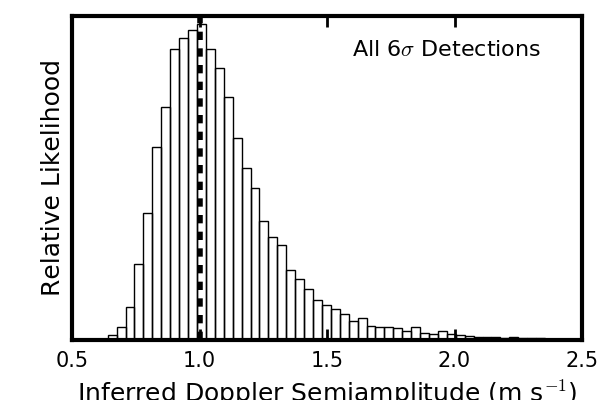
\includegraphics[width=.3\textwidth]{f1.png}\hfill
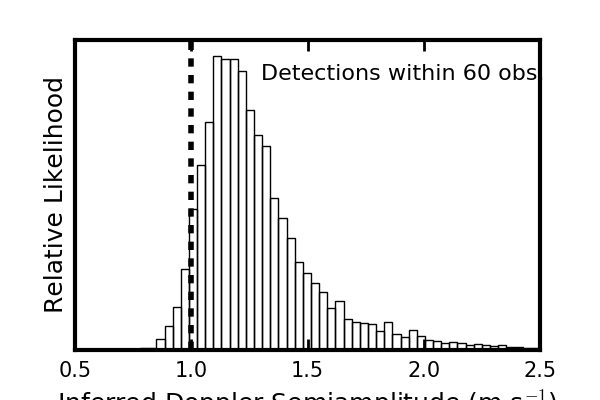
\includegraphics[width=.3\textwidth]{f2.png}\hfill
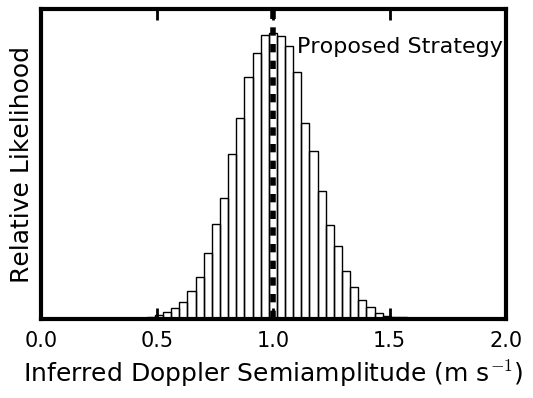
\includegraphics[width=.3\textwidth]{f3.png}

\caption{Inferred mass of a population of planets which induce a 1 m s$^{-1}$ Doppler signal on their host star. (Left) Mass distribution for planets observed until their mass is deemed significant at the $6\sigma$ level. (Center) The same, only including planets with significant mass measurements within 60 epochs. 95\% of masses are overestimated, 57\% at the $1\sigma$ level. (Right) Mass distribution when a criterion to end observing is determined before obtaining data based on the expected signal for the planet. In this scenario, the observed mass distribution is unbiased.}
\label{fig}

\end{figure}

Therefore, any observing strategy that only publishes planet masses once they reach a certain significance threshold will bias population studies of planet densities and compositions unless they also publish their non-detections and their internal criteria for selecting when to observe---and when to stop observing---targets.

This effect can be ameliorated if, instead of observing until a certain fractional mass precision is achieved, a star is observed until a particular absolute mass precision is achieved. 
From assumptions of a planetary mass-radius relation, an estimate can be made of the expected RV signal before any observations are made \citep[e.g.][]{Chen17}. If the above simulation is repeated, but carried out such that all stars are observed until the Doppler semiamplitude is measured to a precision of 0.16 m s$^{-1}$, or 16\% of the \textit{a priori} RV signal, any overestimate of $\hat{M}$ at any given time cannot affect the choice to continue observing, and this bias disappears. In this case, an inferred mass of $\hat{M} = M + \delta M$ or $\hat{M} = M - \delta M$ is still equally likely, but observing decisions will not be made based on that measurement. When we restrict ourselves to the stars with a significant mass measurement within 60 epochs, then the results are unchanged and the bias is still removed.

Regardless of observing strategy, observing teams should also be encouraged to continue to observe targets after a fractional precision is achieved, and to publish their observing criteria for each star as well as their planet non-detections. If stars are only observed until planet signals are detected at the 6$\sigma$ level (or any arbitrary fractional precision), the first bona fide Earth mass planet to be observed is more likely to be initially interpreted as having a composition similar to Mercury than Earth.




\acknowledgments

I thank Megan Bedell for being great \textbf{Megan: please feel free to suggest something over the top here}, and the University of Chicago Exoplanet Journal Club for conversations that inspired this note. This work was performed under contract with the Jet Propulsion
Laboratory (JPL) funded by NASA through the Sagan Fellowship Program executed
by the NASA Exoplanet Science Institute.

\software{%
  numpy \citep{numpy},
  matplotlib \citep{matplotlib},
  scipy \citep{scipy},
  jupyter \citep{jupyter}
  }

\bibliography{exopapers}


\end{document}
